% \documentclass[bwprint]{cumcmthesis} %去掉封面与编号页
\documentclass[withoutpreface,bwprint]{cumcmthesis} %去掉封面与编号页
\newcommand{\diff}{\mathop{}\!\mathrm{d}} % 正体微分符号

\usepackage{graphicx}       % 用于插入图片
\usepackage{subcaption} 
\usepackage{algorithm}
\usepackage{algorithmic} % 导言区需添加这两个宏包
\usepackage{comment}  

\usepackage{booktabs}
\usepackage{tabularx}
\usepackage{float}
\usepackage[numbers]{natbib}

\title{基于长短期记忆网络(LSTM)的蔬菜补货与定价决策模型}
\tihao{A}
\baominghao{1234}
\schoolname{XX大学}
\membera{yby}
\memberb{hyx}
\memberc{ssh}
\supervisor{老师}
\yearinput{2025}
\monthinput{08}
\dayinput{29}


\begin{document}

% 标题
\maketitle
\nocite{*}
\bibliographystyle{gbt7714-numerical}

\begin{abstract}
本文

    \textbf{针对问题一,}
你好

    \textbf{针对问题二,}

    \textbf{针对问题三,}

    \textbf{针对问题四,}

    \keywords{'xx'\quad'xx'\quad'xx'\quad'xx'\quad'xx'}
\end{abstract}

% 问题背景与重述
\section{问题重述}

\subsection{问题背景}
"板凳龙",

\subsection{问题提出}
某一板凳龙

\textbf{问题1:}

\textbf{问题2:}

\textbf{问题3:}

% 问题分析
\section{问题分析}

\subsection{问题一分析}

\subsection{问题二分析}

\subsection{问题三分析}

% 模型假设
\section{模型假设}

\begin{enumerate}
    \item ..
    \item ..
    \item ..
\end{enumerate}

% 符号说明
\section{符号说明}
\begin{table}[H]
    \centering
    \caption{模型核心符号说明}
    \label{表标签}
    \begin{tabular}{ccc} 
        \toprule[1.5pt]
        \textbf{符号} & \textbf{说明} & \textbf{单位} \\
        \midrule[1pt]
        $g$ & 品类标识 & - \\
        $n_g$ & 第$g$类品类的样本量 & - \\
        \bottomrule[1.5pt]
    \end{tabular}
\end{table}

% 模型建立与求解
\section{模型建立与求解}
\subsection{问题一的模型建立与求解}
\subsubsection{模型建立}


\begin{figure}[htbp]
    \centering
    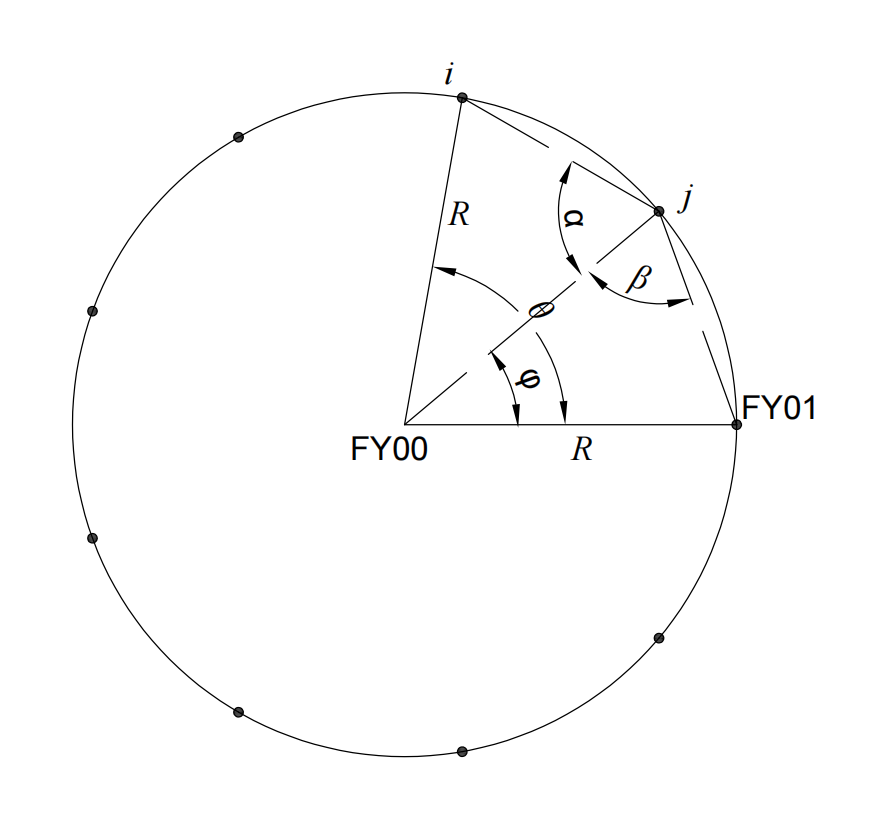
\includegraphics[width=0.6\textwidth]{../../figure/q1_1.png} 
    \caption{主动机与被动机排布的情况1}
    \label{q1_1}
\end{figure}

\begin{figure}[htbp]
    \centering
    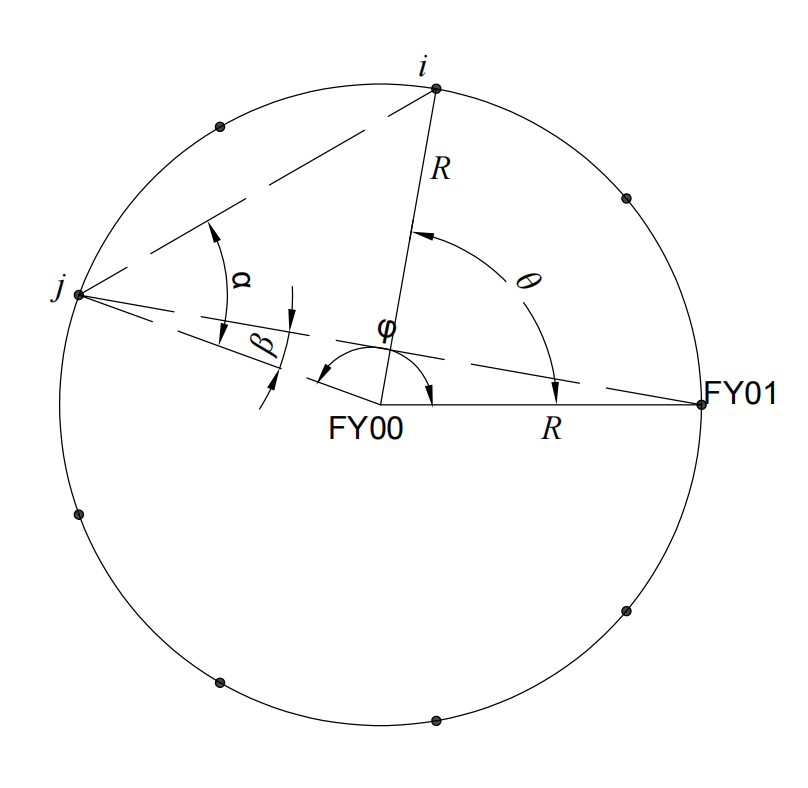
\includegraphics[width=0.6\textwidth]{../../figure/q1_2.png} 
    \caption{主动机与被动机排布的情况2}
    \label{q1_2}   
\end{figure}

\begin{figure}[htbp]
    \centering
    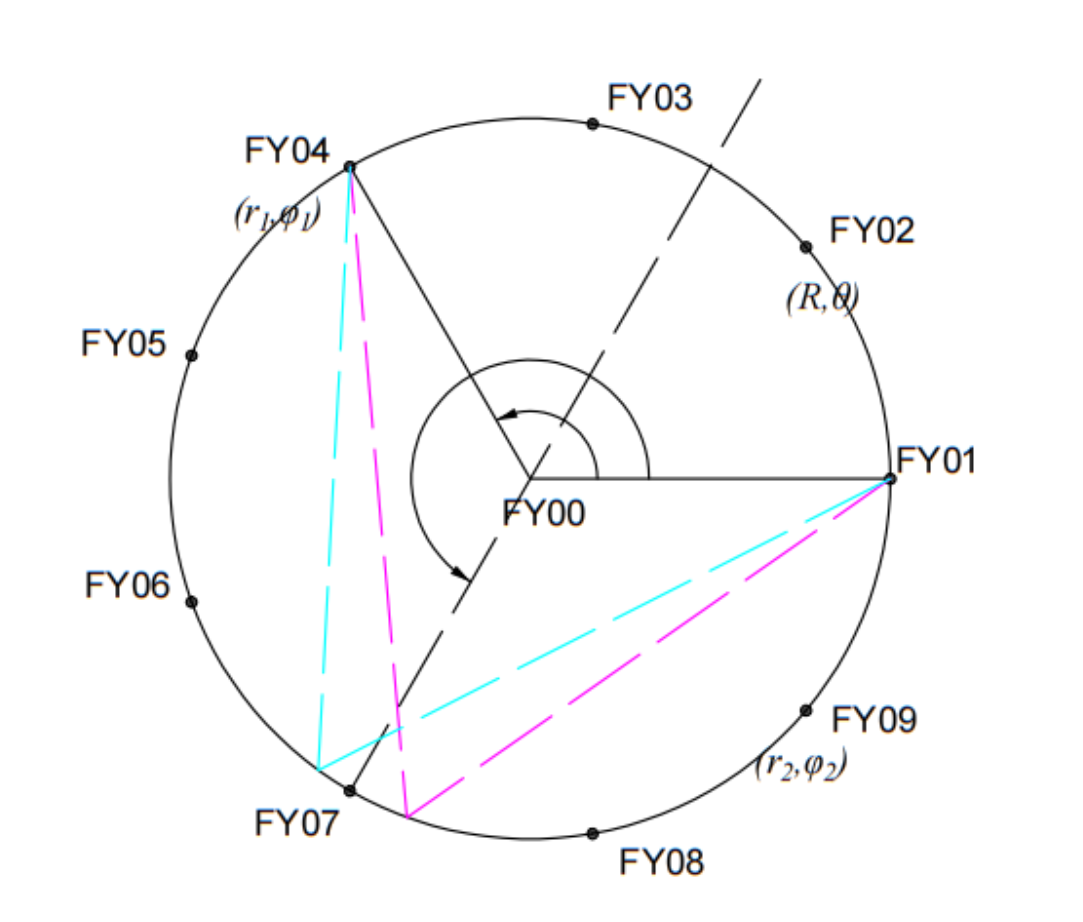
\includegraphics[width=0.95\textwidth]{../../figure/q1_4.png} 
    \caption{方案一对应的流程图}  
    \label{q1_4}    
\end{figure}

\begin{figure}[htbp]
    \centering
    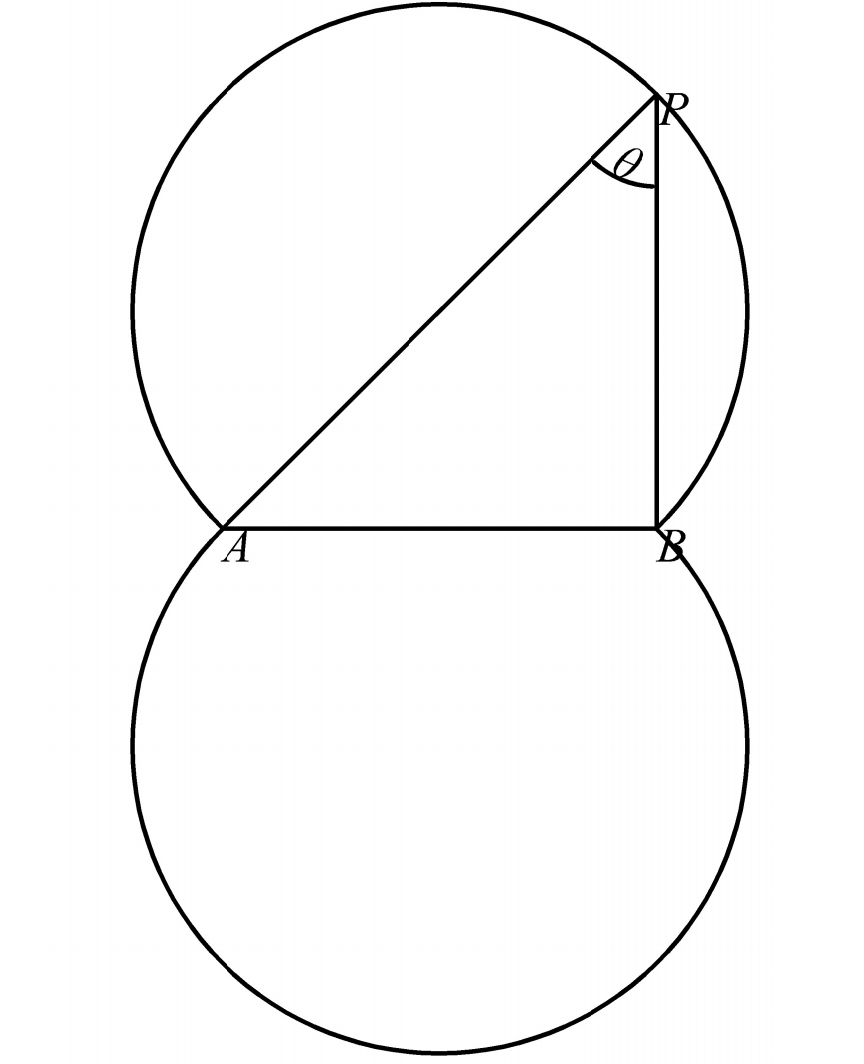
\includegraphics[width=0.6\textwidth]{../../figure/q1_3.png} 
    \caption{哈哈}
    \label{q1_3}   
\end{figure}

\subsubsection{问题求解}
\subsubsection{求解结果}

\subsection{问题二的模型建立与求解}
\subsubsection{模型建立}
\subsubsection{问题求解}
\subsubsection{求解结果}

\subsection{问题三的模型建立与求解}
\subsubsection{模型建立}
\subsubsection{问题求解}
\subsubsection{求解结果}

% 模型的分析与检验
\section{模型的分析与检验}
\subsection{误差分析}
\subsection{灵敏度分析}


% 模型评价
\section{模型的评价}
\subsection{模型优点}
\begin{enumerate}
    \item ..
    \item ..
    \item ..
\end{enumerate}

\subsection{模型缺点}
\begin{enumerate}
    \item ..
    \item ..
\end{enumerate}

\subsection{改进方向}
\begin{enumerate}
    \item ..
    \item ..
\end{enumerate}

% 摘要
\bibliography{ref}

% 附录

\begin{appendices}

\section{运行结果}


\section{文件列表}
\begin{table}[H]
    \caption{程序文件列表}
    \centering
    \begin{tabularx}{\textwidth}{l X}
        \bottomrule
        文件名 & 功能描述 \\
        \midrule
        Enums.py & 自定义枚举类型 \\
        SaleFlow.py & 处理文档,将附件2的流水整理为便用的形式 \\
        SaleUtils.py & 处理表格、绘图等工具 \\
        code1.py & 问题一程序代码 \\
        code2.py & 问题二程序代码 \\
        code3.py & 问题三程序代码 \\
        \bottomrule
    \end{tabularx}
    \label{tab:文件列表}
\end{table}

\section{代码}
问题1代码
\lstinputlisting[language=python]{../../code/code1.py}
问题2代码
\lstinputlisting[language=python]{../../code/code2.py}
问题3代码
\lstinputlisting[language=python]{../../code/code3.py}

\end{appendices}

\end{document}